\chapter{State-Space Aggregation}\label{ch:lumping}
\section{Macro-States}
A macro-state is a collection of micro-states (or simply states) treated as one state in the aggregated model, which can be seen as an abstraction of the original model.
The aggregation scheme defines a partitioning of the state-space.
We choose a scheme based on a grid structure. That is, each macro-state is a hypercube in $\mathbb{Z}_{\geq 0}^{n_S}$.

Hence, each macro-state $\bar{x}_i(\ell^{(i)},u^{(i)})$ (denoted by $\bar{x}_i$ for notational ease) can be identified using two vectors $\ell^{(i)}$
and $u^{(i)}$.
The vector $\ell^{(i)}$ gives the corner closest to the origin, while $u^{(i)}$
gives the corner farthest from the origin.
Formally,
\begin{equation}\label{eq:macros_state}
    \bar{x}_i = \bar{x}_i(\ell^{(i)},u^{(i)}) =  \{x\in\mathbb{N}^{n_S} \mid  \ell^{(i)}  \leq x  \leq u^{(i)} \},
\end{equation}
where '$\leq$' denotes element-wise comparison.

In order to solve the aggregated model, we need to define transition rates between macro-states.
Therefore, we assume that, given that the system is in a particular macro-state, all constituent states are equally likely (uniformity assumption).
This assumption is the reason why the aggregated model provides only a coarse-grained approximation. 

The uniformity assumption is a modeling choice yielding significant advantages.
Firstly, it eases the computation of the rates between macro-states and, therefore, makes a fast solution of the aggregated model possible.
Secondly, even though it induces an approximation error, it provides suitable guidance as uniformity assumption spreads out the probability mass conservatively.
Hence, it becomes less likely that regions of interest are disregard.
Lastly, the uniformity assumption is theoretically well-founded, as it stems from the maximum entropy principle: 
In the absence of concrete knowledge about the probability distribution inside a macro-state, we assume the distribution with the highest uncertainty, i.e., the uniform distribution. 

\section{Construction}
The grid structure makes the computation of transition rates between macro-states particularly convenient and computationally simple.
Mass-action reaction rates can be given in a closed-form,
due to the Faulhaber formulae~\cite{knuth1993johann} and more complicated rate functions such as Hill-functions can often be handled as well by taking appropriate integrals (see \autoref{sec:bridging:hill_toggle}).

Suppose, we are interested in the transition rate from macro-state $\bar{x}_i$ to macro-state $\bar{x}_k$ according to reaction $j$.
Using the uniformity assumption, this is simply the mean rate of the states in $\bar{x}_i$ that go to $\bar{x}_k$ using $j$.
However, only a small subset of constituents in $\bar{x}_i$ are actually relevant for this transition.
Hence, we identify the subset of states of $\bar{x}_i$ that lie at the border to $\bar{x}_k$ and in such a way that applying reaction $j$ shifts them to a state in $\bar{x}_k$. Then, we sum up the corresponding rates of these states. Lastly, we normalize according to the number of states inside of $\bar{x}_i$.

It is easy to see that the relevant set of border states is itself an
interval-defined macro-state $\bar{x}_{i\xrightarrow{j}k}$.
To compute this macro-state
we can simply shift $\bar{x}_i$ by $v_j$, take the intersection
with $\bar{x}_k$ and project this set back.
Formally,
\begin{equation}\label{eq:transition_set}
    \bar{x}_{i\xrightarrow{j}k} = ((\bar{x}_i + v_j) \cap \bar{x}_k) - v_j\,,
\end{equation}
where the additions are applied element-wise to all states
making up the macro-states.
For ease of notation, we also define a general exit state
\begin{equation}
    \bar{x}_{i\xrightarrow{j}} = ((\bar{x}_i + v_j) \setminus \bar{x}_i) - v_j.
\end{equation}
This state captures all micro-states inside $\bar{x}_i$ that can leave the state via reaction $j$.

This uniformity assumption gives rise to the following $Q$-matrix of the aggregated model:
\begin{equation}\label{eq:lumped_q}
    \bar{Q}_{ \bar{x}_i,  \bar{x}_k} = \begin{cases}
        \sum_{j=1}^{n_R}{\bar\alpha}_j\left(\bar{x}_{i\xrightarrow{j}k}\right)/\left|\bar{x}_i\right|\,,&\text{if}\; \bar{x}_i\neq \bar{x}_k\\[1ex]
        -\sum_{j=1}^{n_R}{\bar\alpha}_j\left(\bar{x}_{i\xrightarrow{j}}\right)/{\left|\bar{x}_i\right|}\,, &\text{otherwise}
    \end{cases}
\end{equation}
where 
\begin{equation}\label{eq:lumped_propfun}
    \bar{\alpha}_j({\bar{x}}) = \sum_{x\in \bar{x}} \alpha_j(x).
\end{equation}
is the sum of all rates belonging to reaction $j$ in $\bar{x}$.



Under the assumption of polynomial rates, as is the case for mass-action
systems, we can compute the sum of rates over this transition set
efficiently using Faulhaber's formula.
As an example consider the following mass-action reaction
$ 2 X \xrightarrow{c} \varnothing\,. $
For macro-state
$\bar{x} = \{0, \dots, n\}$
we can compute the corresponding lumped transition rate
$$\bar{\alpha}(\bar{x})
=\frac{c}{2}\sum_{i=1}^n i (i - 1)
=\frac{c}{2}\sum_{i=1}^n (i^2 - i)
=\frac{c}{2}\left(\frac{2n^3+3n^2+n}{6} - \frac{n^2 + n}{2}\right)$$
eliminating the explicit summation in the lumped propensity function.

Interestingly, the lumped distribution
tends to be less concentrated. %\MB{rephrase this passage in terms of entropy?}\todo{L: this is interesting, but why? maybe an intuition of why uniform spreads more the distribution}
This is due to the assumption of a
uniform distribution inside macro-states.
This effect is illustrated by the example of a birth-death process in \autoref{fig:lumped} and \autoref{fig:lumped_terminal}.
Due to this effect, an iterative refinement typically keeps an over-approximation in terms of state-space area.
This is a desirable feature since relevant regions are less likely to be pruned due to lumping approximations.
\begin{figure}
    \centering
    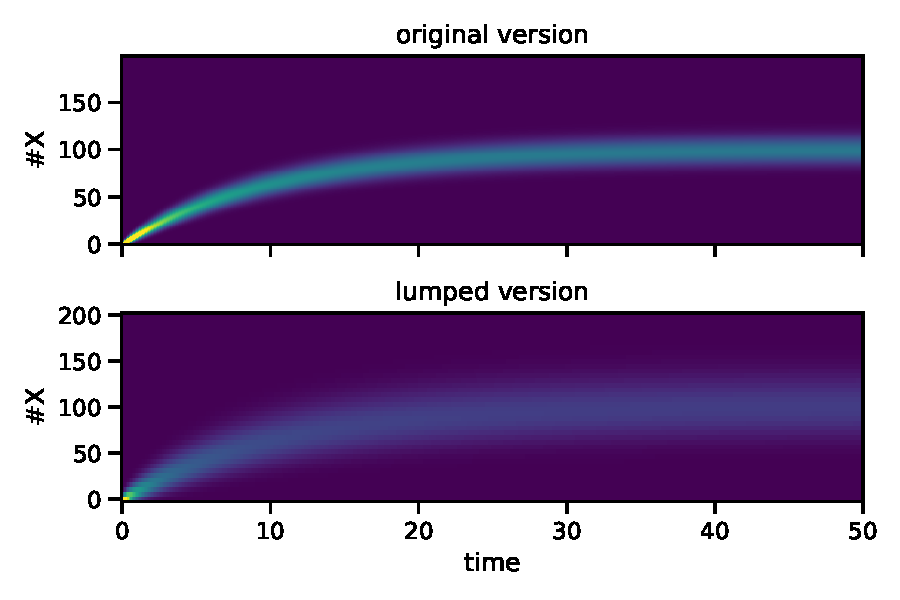
\includegraphics[scale=.6]{gfx/lumpedvorig.pdf}
	\caption[Lumping approximation of \autoref{model:bd}]{A lumping approximation of \autoref{model:bd} on the state-space truncation to $[0, 200]$ on $t\in[0, 50]$. On the left-hand side solutions of a regular truncation approximation and a lumped truncation (macro-state size is 5) are given.}
    \label{fig:lumped}
\end{figure}
\begin{figure}
    \centering
    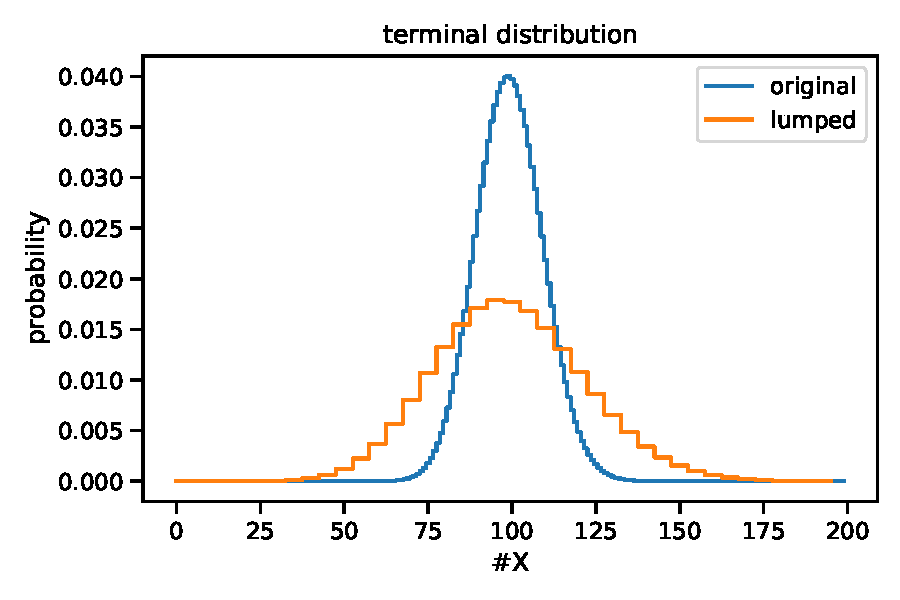
\includegraphics[scale=.6]{gfx/lumped_dist.pdf}
	\caption[Distribution of a lumped approximation]{The terminal distributions $\Pr(X_{50}=x_i)$ of a lumped approximation and a truncation at original granularity are given.}
    \label{fig:lumped_terminal}
\end{figure}
